\documentclass[17pt]{beamer}

\usepackage[utf8]{inputenc}
\usepackage{listings}
\usepackage{tikz}
\usetikzlibrary{positioning}
\usetikzlibrary{arrows.meta}
\usepackage{pgfplots}
\pgfplotsset{compat=1.16}
\usepackage{inconsolata}

%\usepackage{pgfpages}
%\setbeameroption{show notes on second screen=left}

% presentation themeing
\usetheme{Singapore}
\beamertemplatenavigationsymbolsempty
\setbeamertemplate{bibliography item}{\insertbiblabel}

% Julia listings definition
% Definition based on https://tex.stackexchange.com/a/212794/149437
\lstdefinelanguage{Julia}
  {otherkeywords={::},
   keywords=[1]{::,abstract,break,case,catch,const,continue,do,else,elseif,
      end,export,for,function,immutable,import,importall,if,in,
      macro,module,otherwise,quote,return,switch,try,type,typealias,
      using,while,where},
   keywords=[2]{false,true},
   sensitive=true,
   alsoother={$},
   morecomment=[l]\#,
   morecomment=[n]{\#=}{=\#},
   morestring=[s]{"}{"},
   morestring=[m]{'}{'},
}[keywords,comments,strings]


\title[JuliaPetra]{Obtaining Performance from a Julia-Implementation of Trilinos Data Libraries}
\author{Neil Lindquist}
\institute{Saint John's University, Minnesota}
\date[SIAM CSE19]{\small SIAM Conference on Computational Science and Engineering\\February 27th 2019}


\begin{document}
\frame{\titlepage}
\begin{frame}
	\frametitle{Julia}
	\nocite{Bezanson:2017:FreshApproach}
	\begin{itemize}
		\item High Level
		\item Compiles to efficient machine code
	\end{itemize}
	%TODO consider if Wilkins prize should be mentioned
	%TODO should LLVM be mentioned?
	\note{
		high level language
		
		can perform on par with C
		\begin{itemize}
			\item type inferencing
			\item compiling each concrete method signature
		\end{itemize}
		
		investigating whether Julia is usable for distributed, high performance codes
	}
\end{frame}

\begin{frame}
	\frametitle{Petra Object Model}
	\nocite{Heroux:2005:Trilinos}
	\begin{itemize}
		\item Family of sparse linear algebra frameworks
		\item Underlying data libraries for Trilinos
		\item 3 existing implementations
	\end{itemize}
	\note{
		The Petra libraries are the underlying data structures used by Trilinos
		
		3 implementations
		\begin{itemize}
			\item Epetra - original, portable version
			\item Tpetra - newer, uses more advanced C++ features
			\item Jpetra - experiemental, pure java version
		\end{itemize}
	}
\end{frame}
\begin{frame}
	\frametitle{JuliaPetra Organization}
	\nocite{Github:MPI}
	\centering
	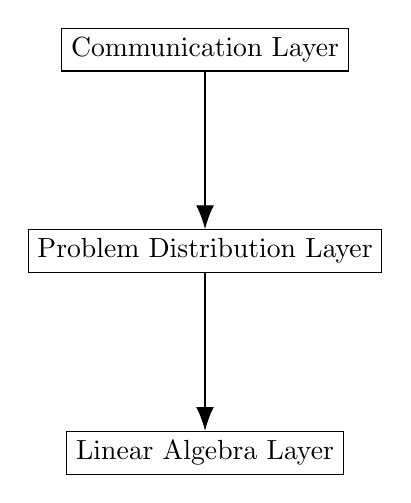
\begin{tikzpicture}
		\node[rectangle, draw=black] (CommLayer) {Communication Layer};
		\node[rectangle, draw=black] (DistLayer) [below=2cm of CommLayer] {Problem Distribution Layer};
		\node[rectangle, draw=black] (LALayer) [below=2cm of DistLayer] {Linear Algebra Layer};
		\draw[-{Latex[length=3mm]}] (CommLayer.south) -- (DistLayer);
		\draw[-{Latex[length=3mm]}] (DistLayer.south) -- (LALayer);
	\end{tikzpicture}
	\note{
	Communication layer handles the movement of data between processes
	\begin{itemize}
		\item Can be implemented with any Single-Program-Multiple-Data parallel system
		\item There are serial and MPI implementations
		\item MPI.jl is used for MPI communication
	\end{itemize}
	Distribution layer managed how the parts of the problem are distributed
	
	Linear Algebra layer provides the iterfaces for vector and linear transformation objects
	}
\end{frame}
\begin{frame}[fragile]
	\frametitle{JuliaPetra Example}
	%TODO should only part of the snippet be here for better absorbability?
	\begin{lstlisting}[
		language         =Julia,
		basicstyle       =\ttfamily,
		keywordstyle     ={[1]\bfseries\color{black}},
		keywordstyle     ={[2]\color{blue}},
		stringstyle      =\color{red},
		commentstyle     =\color{gray},
		showstringspaces =false,
		mathescape
		]
apply!(z, A, q)
$\lambda$ = dot(q, z)[1]
@. r = z - $\lambda$*q
	\end{lstlisting}
	\note{
		Here is an example of JuliaPetra.
		
		This is a few lines from the power method for finding eigenvalues
		
		Note that greek letters are allowed in the source
		\begin{itemize}
			\item vector symbol is also allowed, but latex has issues with compiling it
		\end{itemize}
	}
\end{frame}
\begin{frame}
	\frametitle{Performance Comparison}
	\nocite{Github:DA,Gu:2000:PowerMethod}
	\centering
	%TODO this graph doesn't really show that much.  Change to ratio instead?
	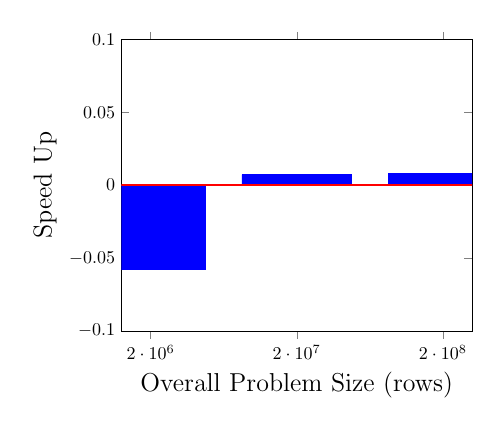
\begin{tikzpicture}[scale=0.65]
		\begin{axis}[
			xlabel = {\Large Overall Problem Size (rows)},
			xtick = {6,7,8},
			xticklabels = {\(2\cdot10^6\), \(2\cdot10^7\), \(2\cdot10^8\)},
			ybar,
			bar width = .75,
			ylabel = {\Large Speed Up},
			ymin  = -0.1,
			ymax  = 0.1,
			yticklabel style={/pgf/number format/fixed},
			]
			\addplot[blue,fill=blue] coordinates{(6,-0.0576)(7,0.0072)(8,0.0080)};
			\addplot[very thick,red,sharp plot,update limits=false] coordinates{(5,0) (9,0)};
		\end{axis}
	\end{tikzpicture}
	
	JuliaPetra Time over Epetra Time.
	\note{
		Latency speed up of JuliaPetra over Epetra
	
		Results are for a tridiagonal matrix using a 20 core machine
	
		DistributedArrays.jl was significantly slower
	}
\end{frame}
\begin{frame}
	\frametitle{Optimizing JuliaPetra}
	\begin{itemize}
		\item Requires disabling high level features
		\begin{itemize}
			\item Dynamic Typing
			\item Garbage Collection
			\item Bounds Checks
		\end{itemize}
	\end{itemize}
	\note{
		Because Julia is a high level language, critical sections need to remove some high level features to perform efficiently.
		
		There are 3 main sets of high level features that I needed to work around
		\begin{itemize}
			\item Dynamic typing
			\item Garbage collection
			\item Bounds checks
		\end{itemize}
	}
\end{frame}
\begin{frame}
	\frametitle{Type Stability}
	\framesubtitle{Optimizing JuliaPetra}
	\begin{itemize}
		\item Julia supports dynamically typed code
		\item When variable types can be inferred, code is ``Type Stable''
		\item Allows function calls to be inlined
	\end{itemize}
	\note{
		Because Julia supported dynamically typed code, ensuring that the compile can deduce the types of each value is very important for performant code
		
		This is called type stability.
		
		Type stable code allows the compiler to figure out which method instance must be called for each function call which reduces the method dispatch overhead and is a requirement for inlining.
		\begin{itemize}
			\item Because Julia implements almost all operations as function calls, inlining is absolutely critical for code to perform efficiently.
		\end{itemize}
		
		Julia does compile functions for each set of leaf types that it is called with, to help with type stability.
	}
\end{frame}
\begin{frame}
	\frametitle{TypeStability Tools}
	\framesubtitle{Optimizing JuliaPetra}
	\nocite{Github:TypeStability.jl}
	\begin{itemize}
		\item \texttt{code\_warntype} - view deduced types in code
		\item TypeStability.jl - Automate type stability checks
	\end{itemize}
	\note{
		Because type stability is so important to performance, tools to ensure code is type stable are crucial when optimizing
		
		code\_warntype is a built in function to manually inspected the results of type inferencing and inlining.
		
		However, checking that a function behaves for different sets of arguments is very tedious.
		
		To automate type stability checks, I created a basic package, TypeStability.jl.
	}
\end{frame}
\begin{frame}
	\frametitle{Reducing Garbage Collection}
	\framesubtitle{Optimizing JuliaPetra}
	\begin{itemize}
		\item Garbage collection is automatic
		\item \texttt{Ptr} type doesn't need garbage collection
	\end{itemize}
	\note{
		Garbage collection is automatic
		
		Only immutable objects that don't reference heap allocated objects can be allocated with the stack for cheap deallocation.
		
		Matrix vector product requires heavy use of array views.
		
		Used a pointer type from the C interface to prevent heap allocating views.
		
		This trick only works were original array is safe from garbage collection
	}
\end{frame}
\begin{frame}
	\frametitle{Bounds Checks}
	\framesubtitle{Optimizing JuliaPetra}
	\begin{itemize}
		\item Julia checks bounds automatically
		\item \texttt{@inbounds} macro skips bounds checks
	\end{itemize}
	\note{
		Julia checks boundaries by default
		
		Want to eliminate those checks when known to be unnecessary
		
		Julia has a \texttt{inbounds} macro to indicate that bounds checks aren't needed
		\begin{itemize}
			\item Only honored when bound check is inlined into the calling method.
		\end{itemize}
	}
\end{frame}
\begin{frame}
	\frametitle{Conclusion}
	\begin{itemize}
		\item Julia is a promising fast, high level language
		\item JuliaPetra matches Epetra's performance
		\item Optimizing Julia requires disabling some high level features
	\end{itemize}
	\note{
		Julia is fast and high level
		
		JuliaPetra matches Epetra
		
		Optimizing Julia requires eliminating the overhead of some high level features
	}
\end{frame}
\begin{frame}[allowframebreaks]
	\frametitle{References}

	\bibliographystyle{siam}
	\small\bibliography{bibliography}

\end{frame}
\end{document}
